% Revision 5 candidate: complete numerical, visual and independent paper review records are external.
% Preserve the recorded recommendations and all original experimental outcomes.
\documentclass[conference]{IEEEtran}
\usepackage{amsmath,amssymb,graphicx,booktabs,array,url}
\usepackage[hidelinks]{hyperref}
\newtheorem{theorem}{Theorem}
\newtheorem{proposition}{Proposition}
\newcommand{\E}{\mathbb{E}}
\newcommand{\C}{\mathcal{C}}
\newcommand{\R}{\mathbb{R}}
\newcommand{\qbridge}{Q-BRIDGE}
\title{Q-BRIDGE: Reusable Policy Certificates across Observational and Randomized Logs}
\hypersetup{pdftitle={Q-BRIDGE: Reusable Policy Certificates across Observational and Randomized Logs},
pdfauthor={Zida Yang, Weiqing Zeng, Guquan You, Cong Wang, Jiexin Zheng}}
% Latest user-confirmed order and roles: only Cong Wang and Jiexin Zheng correspond.
\author{
\IEEEauthorblockN{\href{https://orcid.org/0009-0000-2386-2533}{Zida Yang}$^{1,\dagger}$,
\href{https://orcid.org/0009-0003-0186-6199}{Weiqing Zeng}$^{2,\dagger}$,
\href{https://orcid.org/0009-0005-5915-7058}{Guquan You}$^{3,\dagger}$,
\href{https://orcid.org/0000-0002-5300-0122}{Cong Wang}$^{1,*}$,
\href{https://orcid.org/0009-0005-5838-0135}{Jiexin Zheng}$^{1,*}$}
\IEEEauthorblockA{$^{1}$Guanghua School of Management, Peking University}
\IEEEauthorblockA{$^{2}$Southwest Jiaotong University}
\IEEEauthorblockA{$^{3}$Institute of Emergency Safety Innovations, Guangzhou University}
\IEEEauthorblockA{2401111090@stu.pku.edu.cn, zengweiqing@my.swjtu.edu.cn, youguquan@gzhu.edu.cn}
\IEEEauthorblockA{\{wangcong,jiexinzheng\}@gsm.pku.edu.cn}
\IEEEauthorblockA{$\dagger$ Equal contribution. \quad $*$ Corresponding authors.}
}

\begin{document}
\maketitle
\begin{abstract}
Policy analysts repeatedly compare candidates using the same observational log and randomized experiment. Hidden confounding and population differences limit what these sources can justify. Q-BRIDGE materializes a confidence view from source aggregates and declared transfer of action-group means. One coverage event supports later linear policy queries, including adaptive ones; exact evidence distinguishes certified improvement, a failed robust threshold, and an undecided answer. Statistical claims map explicitly to the stored coefficients checked by each proof. A factorial execution study holds candidate order, answers and solver paths fixed. On three 1,000-query streams from one 512-cell view, retaining exact terms reduces joint producer and receiver time by 24--40\%, depending on screening. Screening saves 10--11\% before retention but costs 12--14\% afterward. In a Coat catalogue workload with ordinary objective caching, further arithmetic optimization saves 4--6\% in the five-view geometric-mean comparison, below its ten-percent target. Information diagnostics separate the gain from added constraints from the cost of dividing a confidence budget; a minimizing-face check identifies zero optimal gain. The 48-world study does not confirm its five-percentage-point target, and the Coat analyses do not certify improvement. These findings distinguish reusable computation from information sufficient to authorize a policy change.
\end{abstract}
\begin{IEEEkeywords}
policy evaluation, causal data integration, materialized views, sensitivity analysis, verifiable computation
\end{IEEEkeywords}

\section{Introduction}
A recommendation team has a production log and a smaller randomized experiment. It repeatedly asks whether a candidate policy improves target success over a reference by a requested margin. Rebuilding confidence intervals and solving a new optimization problem for each candidate repeats shared work. The interface should retain that work and the evidence's limits across the sequence.

Two limits matter. First, unrecorded preferences can affect both production exposure and outcomes. Second, randomization identifies outcomes in the experimental population; it does not establish that every outcome mean transfers to the production target. An analyst may justify transfer only for specified action-group averages. Such information can constrain a target-policy comparison even when the individual action means differ across sources. The query must retain that distinction rather than silently apply full outcome transport.

We study a finite-table interface for binary outcomes. Its \emph{confidence view} stores allowed target cell means and their group constraints for a fixed snapshot and source declaration. Each query supplies two policies and an improvement margin. Checked lower evidence can establish that every allowed mean vector passes; a checked feasible vector can show that the view permits failure. The executor tries saved evidence before computing again. One coverage event supports every objective asked of the same view, including those selected after previous answers.

\textbf{A running example.} Figure~\ref{fig:example} has one context and four actions; $m_A$ is the target success probability under action A. The reference chooses each action with probability $0.25$. Query Q1 moves $0.10$ probability from each of A and B to C and D, giving $c=(-.1,-.1,.1,.1)$. Observational information permits the four mean intervals in the figure. Randomized information transfers only $(m_A+m_C)/2=.65$ and $(m_B+m_D)/2=.70$. Substituting $m_C=1.3-m_A$ and $m_D=1.4-m_B$ yields
\begin{align*}
\Delta_1&=.27-.2(m_A+m_B)\\
&\ge .27-.2(.6+.7)=.01.
\end{align*}
The feasible vector $(.6,.7,.7,.7)$ attains this bound in decimal arithmetic. Thus the worst allowed target still improves success by one percentage point. Neither source alone suffices: the interval-only bound is $-.075$, and the group-only bound is $-.13$. These are constructed teaching inputs, not measured effects.

\begin{figure*}[t]
\centering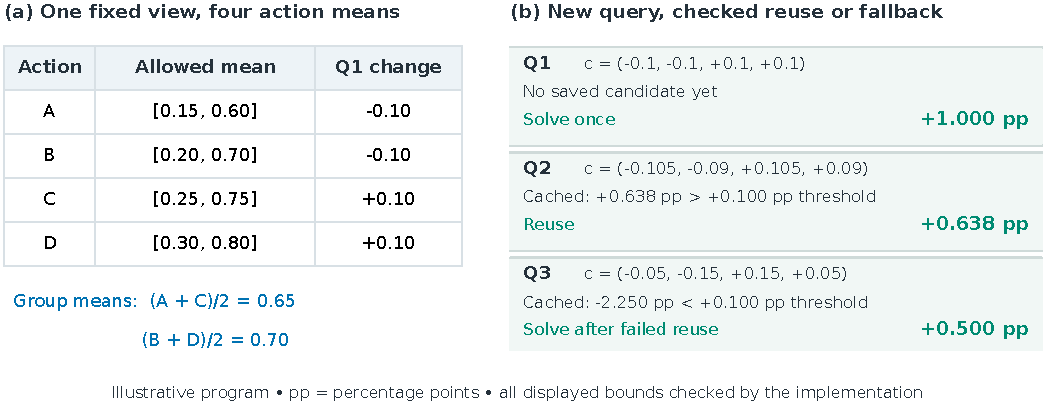
\includegraphics[width=\textwidth]{figures/worked_query_v2.pdf}
\caption{Four target means, one view, three queries. Entries of $c$ change action probabilities; returned bounds concern success-rate improvement in percentage points (pp). Q1 solves, Q2 reuses checked information, and Q3 solves after reuse fails. Displayed values are rounded for readability; exported proofs retain the checked numerical bounds. This is an illustrative program.}
\label{fig:example}
\end{figure*}

Q2 changes the contrast to $(-.105,-.09,.105,.09)$. A saved lower-bound candidate already proves $0.006375$, above the requested $0.001$ margin. Finding Q2's best bound, $0.0105$, is unnecessary for this decision. For Q3, $(-.05,-.15,.15,.05)$, the saved candidate gives $-.0225$; solving produces $0.005$. Failed reuse triggers computation, not a negative policy conclusion. Section~\ref{sec:execution} explains the dual information behind these candidates.

These operations use established sensitivity bounds, simultaneous inference, robust optimization and verified dual reuse~\cite{dorn2025dvds,ishikawa2026convex,Berk2013PoSI,Bertsimas2018DataRobust,Neumaier2004SafeBounds,Marcucci2021WarmStart}. Q-BRIDGE makes their source-to-proof contract explicit: the source declaration determines allowed means, while normalization, interval mapping and numerical checks determine the stored problem each proof certifies. Policies and margins may change under the same coverage event; a new target, source snapshot or statistical declaration requires a new view.

We evaluate two questions. Does evidence reuse reduce total producer-and-receiver work? Does source fusion justify a policy change that neither source alone supports? A factorial execution study holds answers and solver paths fixed while varying screening and retained exact terms. A catalogue workload adds ordinary objective caching and an optimized arithmetic reference. These comparisons test whether avoiding a check still pays after that check becomes cheaper.

The information study separates the gain from adding randomized constraints from the cost of allocating confidence to them, which widens the observational box. Fusion helps only when the gain exceeds that cost. A feasible point on the box's minimizing face proves zero optimal gain. Together with exact finite/population optima, this diagnostic explains the saved certification failures. The scope remains a declared sensitivity relaxation; these computations do not establish a confounding radius from data alone.

\section{The Query and Its Statistical Contract}\label{sec:contract}
\subsection{Target, tables, and declarations}
Let $X\in\{1,\ldots,K\}$ denote a context, $A\in\{1,\ldots,L\}$ an action, and $Y\in\{0,1\}$ an outcome; write $d=KL$. Source $O$ is observational and source $R$ randomized. The unknown target means are $m^O_{xa}=\E_O[Y(a)\mid X=x]$, while $m^R_{xa}=\E_R[Y(a)\mid X=x]$ refers to the experimental population. For specified context weights $w$, policy $\pi$, and reference $\pi_0$, the target contrast is
\begin{equation}
 \Delta(c)=\sum_{x,a}w_x(\pi_{xa}-\pi_{0,xa})m^O_{xa}=c^\top m^O.\label{eq:query}
\end{equation}
Each policy row and $w$ are probability distributions. Policies are encoded as $c$ before execution; the proof binds this coefficient vector and the requested margin. The reference is specified by the caller, not an unknown natural logging policy. Uncertainty in an estimated target-population distribution is outside this contract.

The view stores $\ell\le m\le u$ and $a\le Tm\le b$ for the $d$ target means. In the example, $T$ selects A/C and B/D with weight one half each. Sections~\ref{sec:view} and~\ref{sec:execution} construct and query this fixed object.

The event tables contain iid units $(x,a,y)$ within each source. Repeated ratings require a unit-level treatment (Section~\ref{sec:coat}). Let $N^s_{xay}$ be the cell counts, $N^s_{xa}=\sum_yN^s_{xay}$, and $S^s_{xa}=N^s_{xa1}$. In source $R$, random assignment means $A\perp Y(a)\mid X$ for every action. Its design $q_{xa}=P_R(A=a\mid X=x)$ must be known and positive on the declared moment supports. The two source samples may be dependent, as may moment rows; the confidence construction uses a union bound rather than independence between those intervals.

Before inference, the caller fixes the context mapping, target population, source assumptions, moment rows, sensitivity parameters and confidence allocation, possibly using an independent design sample. The contract conditions on this design. Later objectives and thresholds may adapt to earlier answers; selecting a new snapshot or confidence construction after inspecting inference outcomes needs an additional guarantee.

\subsection{Observational information without a fitted logger}
Write $p_{xa}=P_O(Y=1\mid x,a)$ for the observed success probability among events receiving action $a$. It differs from $m^O_{xa}$, the target mean under that action. Let $U$ collect unobserved factors, and let $e_O(a\mid x,U)$ and $e_O(a\mid x)$ denote conditional and marginal production exposure probabilities. Under consistency, latent conditional ignorability, and latent overlap, a normalized outcome-conditional relative weight satisfies
\begin{align}
 r^*(x,a,y)&=\E_O\!\left[\left.\frac{e_O(a\mid x)}{e_O(a\mid x,U)}\right|x,a,y\right],\nonumber\\
 m^O_{xa}&=\E_O[r^*Y\mid x,a].\label{eq:relative}
\end{align}
The declared sensitivity restriction is $1/\Lambda\le r^*\le\Lambda$, with $\Lambda\ge1$. It bounds the outcome-conditional average $r^*$, not each latent inverse propensity or propensity odds. Neither propensity in~\eqref{eq:relative} is supplied to the implementation. The restriction still requires scientific justification; data alone do not establish a suitable confounding radius~\cite{fawkes2025hardness}.

For binary outcomes the conditional-weight relaxation has the known exact interval image~\cite[Eq.~(9)]{dorn2025dvds}:
\begin{align}
 L_\Lambda(p)&=\max\{p/\Lambda,1-\Lambda(1-p)\},\nonumber\\
 U_\Lambda(p)&=\min\{\Lambda p,1-(1-p)/\Lambda\}.\label{eq:binary}
\end{align}
For $0<p<1$, substituting $r_1=m/p$ and $r_0=(1-m)/(1-p)$ gives these endpoints. Exactness concerns this relaxation, not sharp identification over all compatible latent causal models~\cite{ishikawa2026convex}.

\textbf{Consistency provides additional information.} The same table also implies
\begin{equation}
 P_O(A=a,Y=1\mid x)\le m^O_{xa}\le1-P_O(A=a,Y=0\mid x).\label{eq:consistency}
\end{equation}
These joint-event constraints must enter both fusion and the observational baseline. For example, if an action is chosen with probability $.8$ and $p=.5$, consistency restricts its mean to $[.4,.6]$, whereas the $\Lambda=2$ conditional-weight box alone allows $[.25,.75]$. The stronger constraints are estimable from joint counts; they do not require fitting a propensity function. Section~\ref{sec:historical} shows that this distinction changes a substantive comparison.

\subsection{Which randomized information transfers?}
Each row $j$ selects one context $x_j$, an action subset $S_j$, and nonnegative normalized weights $\nu_{ja}$. Let $H$ contain these ideal weights. The scientific source declaration is
\begin{equation}
 \tau_j=(Hm^R)_j,\qquad |(Hm^O)_j-\tau_j|\le\rho_j.\label{eq:transport}
\end{equation}
The tolerance $\rho_j$ concerns a normalized group mean; it is separate from sampling uncertainty. The declaration permits individual means to differ: changing two means by $(h,-\nu_1h/\nu_2)$ preserves their group average. A policy contrast sensitive to that direction does not transfer in full.

Some policy comparisons depend only on group means; others also depend on unknown differences within a group. With zero tolerance and population moments alone, an unconstrained linear functional is fixed by $Hm$ when its coefficient lies in the row space of $H$. If $c=H^\top v$, then $c^\top m=v^\top\tau$. Conversely, a component of $c$ in the null space of $H$ changes the contrast along that direction wherever the mean box permits movement. Thus group averages need not identify each action, and some queries need no observational information at all. Full cell transport, $H=I_d$ and $\rho=0$, is a stronger special case in which direct randomized policy evaluation is justified. We include this separately declared control in the Coat case instead of handicapping it with a group-only interface.

\section{Building One Confidence View}\label{sec:view}
\subsection{Observational intervals and an explicit budget}
Allocate $\alpha_O$ to the observational source. Half pays for $d$ two-sided Clopper--Pearson intervals~\cite{clopper1934binomial} for $p_{xa}$, each with failure probability $\alpha_O/(2d)$. Denote them $[p^-_{xa},p^+_{xa}]$. The remaining half pays for $2d$ one-sided lower intervals for the joint events in~\eqref{eq:consistency}, each at failure probability $\alpha_O/(4d)$ and with denominator $N^O_x=\sum_{a,y}N^O_{xay}$. Write these lower endpoints $g^1_{xa}$ and $g^0_{xa}$. Then
\begin{align}
 \ell_{xa}&=\max\{L_\Lambda(p^-_{xa}),g^1_{xa}\},\nonumber\\
 u_{xa}&=\min\{U_\Lambda(p^+_{xa}),1-g^0_{xa}\}.\label{eq:obox}
\end{align}
Both binary-image endpoints are monotone, so this propagation is conservative. Conditional binomial intervals permit random stratum counts under the stated iid sampling model. Empty action cells contribute $[0,1]$ to the conditional part; empty contexts contribute no joint-event restriction. No missing mean is filled in with a point estimate. Dependence among the intervals does not change their union-bound budget.

\subsection{Two prespecified randomized constructions}
Allocate $\alpha_R$ to the randomized source. We implement two separately calibrated alternatives, selected before examining their inference outcomes.

\textbf{Projected cell intervals.} Construct simultaneous binomial intervals $[r^-_i,r^+_i]$ for every randomized cell appearing in $H$, splitting $\alpha_R$ across those cells. Nonnegativity of $H$ gives normalized group intervals $[Hr^-,Hr^+]$. Only these \emph{group} intervals enter~\eqref{eq:transport}; individual experimental means are not equated to target means. This construction can differ materially in width from the group-score route. Selecting the tighter route after seeing the data is not authorized by either route's individual budget.

\textbf{Group scores.} Conditional on an event falling in $(x_j,S_j)$, define $q_j(a)=q_{x_ja}/\sum_{b\in S_j}q_{x_jb}$ and $Z_j=\nu_{jA}Y/q_j(A)$. Then $\E[Z_j]=\tau_j$ and $0\le Z_j\le B_j=\max_a\nu_{ja}/q_j(a)$. Its count, sum and squared sum are obtained from $N^R_{xay}$, since $Y^2=Y$. If every score multiplier $\nu_{ja}/q_j(a)$ equals one on $S_j$, then $Z_j=Y$ and we use a binomial interval. Otherwise, for $n_j\ge2$, the two-sided empirical Bernstein interval~\cite{maurer2009eb} has half-width
\begin{equation}
 h_j=\sqrt{\frac{2\widehat{\operatorname{Var}}(Z_j)\log(4/\beta_j)}{n_j}}
 +\frac{7B_j\log(4/\beta_j)}{3(n_j-1)}.\label{eq:eb}
\end{equation}
Here $\beta_j=\alpha_R/J$, and the sample variance uses $n_j-1$. Clip the resulting expectation interval to $[0,1]$; for insufficient observations use the full range. Overlapping groups share events but remain covered by the same union bound.

\begin{figure*}[t]
\centering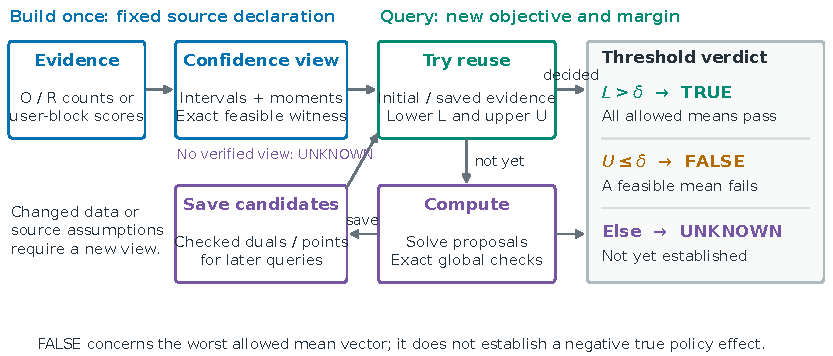
\includegraphics[width=\textwidth]{figures/execution_flow_v3.pdf}
\caption{One view, one three-valued robust threshold query. Lower evidence can prove that every allowed mean passes the margin; an exact feasible point can prove that the view permits a counterexample. Otherwise the verdict remains unknown. A numerical refusal supplies no bound and retains its reason. Producer and receiver independently check evidence against the same trusted view and current objective.}
\label{fig:execution}
\end{figure*}

\subsection{Preserving the statistical meaning in stored coefficients}
The exact proof checker interprets every stored binary64 coefficient as a rational number. A stored row need not sum to exactly one: five stored values of $.2$ sum to $1+2^{-54}$. Treating that row as an exactly normalized average would leave a gap between statistical coverage and the checked program.

For each nonzero stored row $T_j$, define its exact mass $\kappa_j=\sum_iT_{ji}$ and $H_{ji}=T_{ji}/\kappa_j$. This explicitly defines the normalized estimand and gives $T_jm=\kappa_jH_jm$. Zero rows are deterministic zero constraints. Assignment probabilities likewise have declared semantics: either exact probabilities summing to one or explicitly normalized nonnegative design weights. Normalizing a vector does not by itself establish that it describes the data-generating assignment law.

For a covered normalized interval $[\tau_j^-,\tau_j^+]$ and a normalized transport tolerance $\rho_j$, store
\begin{align}
 a_j&=\operatorname{down}\!\left[\kappa_j(\tau_j^- -\rho_j)\right],\nonumber\\
 b_j&=\operatorname{up}\!\left[\kappa_j(\tau_j^+ +\rho_j)\right].\label{eq:represented}
\end{align}
Projected intervals use the exact sums $T_jr^-$ and $T_jr^+$ before subtracting or adding $\kappa_j\rho_j$. Observational endpoint propagation, complements, score moments and normalization are evaluated rationally, then converted outward once at the endpoint. An exact empty interval is refused before conversion, even if rounding would make its endpoints coincide. CP quantiles and the entire floating-point Bernstein half-width kernel, including its arithmetic and log/square-root calls, remain trusted. This mapping does not turn those routines or the scientific declarations into formally verified statistics.

Policy encoding has a separate boundary. If an ideal rational policy contrast $c^*$ is stored as $c$, let $e=c^*-c$. Because $0\le m_i\le1$, a checked bracket $[L,U]$ for the stored objective gives the conservative ideal-policy bracket
\begin{equation}
 [L+\sum_i\min(e_i,0),\ U+\sum_i\max(e_i,0)].\label{eq:policy-rounding}
\end{equation}
The additions and threshold comparison are exact. A positive stored bound alone need not establish a positive ideal contrast at a zero margin. The catalogue workflow retains both representations and their decisions; results for the earlier encoded query families concern their stored contrasts.

\subsection{Coverage and permitted reuse}
Choose $\alpha_O+\alpha_R=\alpha$; fusion uses equal halves in our studies. With endpoints mapped as in~\eqref{eq:represented}, save
\begin{equation}
 \widehat\C=\{m:\ell\le m\le u,\ a\le Tm\le b\}.\label{eq:view}
\end{equation}
The ideal query bound is $V(c)=\min_{m\in\widehat\C}c^\top m$.

\begin{theorem}[One event, all objectives]\label{thm:simultaneous}
Under the source and sampling conditions in Section~\ref{sec:contract}, $P(m^O\in\widehat\C)\ge1-\alpha$. On that event, every linear objective, including one chosen adaptively from previous answers, satisfies $V(c)\le c^\top m^O$. Any verified lower approximation to $V(c)$ shares this inequality. A method that cannot establish a usable view or bound makes no positive assertion.
\end{theorem}
\noindent\textit{Proof.} Condition on independent design information. Each conditional interval has its allocated coverage conditional on its stratum count; averaging over that count preserves the guarantee. A union bound covers all observational conditional and joint-event quantities with probability at least $1-\alpha_O$. Monotonicity and consistency then imply $\ell\le m^O\le u$. The analogous union bound for either prespecified randomized construction covers $Hm^R$ with probability at least $1-\alpha_R$. Adding normalized transport tolerances, multiplying each row by its exact nonnegative mass, and rounding outward yields $a\le Tm^O\le b$. The two source events jointly hold with probability at least $1-\alpha$. On their intersection, minimizing any objective over a set containing $m^O$ cannot exceed its value at $m^O$. This statement holds for all objectives on the same event, so selecting one does not introduce another error event. Weak duality preserves it for lower numerical approximations.\hfill$\square$

The reuse rule is to change queries while retaining the view's statistical design~\cite{Berk2013PoSI,Bertsimas2018DataRobust}. Count-built fusion views store count digests, confidence allocation, assignment design, radius, tolerances and matrix; enclosing protocols retain standalone and fixture provenance. Changing the view or its metadata changes its identity.

\subsection{When group information cannot improve the bound}\label{sec:budget-geometry}
Combining sources narrows a fixed box, but paying for randomized intervals widens the observational box. Write $\mathcal B_{\alpha}$ for full-budget OBS and $\mathcal B_{\alpha/2}$ for the box inside equal-split fusion. Then $\mathcal B_{\alpha}\subseteq\mathcal B_{\alpha/2}$. For nonempty boxes and a nonempty fusion view $\C_F=\mathcal B_{\alpha/2}\cap\{a\le Tm\le b\}$, let $B_{\alpha}$ and $B_{\alpha/2}$ denote the two box minima. The fused optimum satisfies
\begin{equation}
 V_F-B_{\alpha}=\underbrace{(V_F-B_{\alpha/2})}_{G\ge0}
                  -\underbrace{(B_{\alpha}-B_{\alpha/2})}_{P\ge0}.\label{eq:gain-cost}
\end{equation}
Fusion improves the full-budget observational bound exactly when its constraint gain $G$ exceeds its budget cost $P$.

\begin{proposition}[A checkable zero-gain condition]\label{prop:box-face}
Let $F_c=\arg\min_{m\in\mathcal B_{\alpha/2}}c^\top m$. Then $G=0$ if and only if $F_c$ contains a point satisfying all randomized group constraints. If $F_c$ is a singleton, checking its moment rows decides whether $G=0$ or $G>0$.
\end{proposition}
\noindent\textit{Proof.} A feasible box minimizer attains the box lower bound in $\C_F$, proving equality. Conversely, the nonempty compact set $\C_F$ attains its minimum; equality puts an attaining point in $F_c$. If the sets do not intersect, compactness gives a strict gap.\hfill$\square$

This elementary LP criterion supplies a diagnostic before solving a fused program: choose box endpoints by the signs of $c$, then check its group rows. A passing point proves that the additional constraints cannot compensate any positive budget cost. If zero coefficients leave a non-singleton minimizing face, failure of one candidate is inconclusive. The rule concerns the current declared intervals, not whether a future experiment could help. Section~\ref{sec:information-results} applies it to actual certification losses.

\section{Execution with Checkable Answers}\label{sec:execution}
Figure~\ref{fig:execution} follows a request from its trusted view to independently checked evidence. A numerical refusal retains its reason and supplies no bound. Section~\ref{sec:threshold} defines the three-valued decision; proof failure never authorizes a policy change.



\subsection{Sufficient counts and a feasibility gate}
For the independent-event input above, binary score sums and squared sums are linear combinations of $2d$ counters per source. Equal counts and declarations produce equal constraints. Chunked aggregation takes $O(n_O+n_R)$ work and $O(d)$ counter storage apart from its input chunk; new objectives need no further scan. User panels instead require user-level group scores, as detailed in Section~\ref{sec:coat}; item counts alone cannot recover their group-score variance.

Every query requires a feasible point for the entire represented view. The implementation checks a solver proposal and, if needed, a slack-maximizing proposal against all coordinate and moment constraints in exact rational arithmetic. Without a checked witness it returns \texttt{uncertain}; this does not prove emptiness and may refuse difficult zero-volume sets. An empty set cannot bypass this gate with a spuriously large dual value.

\subsection{A lower-bound proof rather than a primal objective}
A feasible primal objective upper-bounds a minimization problem; certification requires a lower bound. For any nonnegative multipliers $\eta_L,\eta_U$, put $z=c+T^\top(\eta_U-\eta_L)$. Weak duality gives
\begin{equation}
 D(c;\eta)=a^\top\eta_L-b^\top\eta_U+
       \sum_i\min\{z_i\ell_i,z_i u_i\}\le V(c).\label{eq:dual}
\end{equation}
Indeed, subtract the lower constraints and add the upper constraints to the objective; their signed terms are nonpositive at every feasible point. Minimizing the remaining linear expression over the box yields~\eqref{eq:dual}. Any nonnegative candidate is valid; optimality only determines its tightness. This is the bounded-variable residual correction underlying reliable LP bounds~\cite{Neumaier2004SafeBounds}.

The checker converts each represented floating coefficient to an exact rational, evaluates the expression, and rounds its final floating result toward negative infinity. It binds the proof to the view's digest, requested objective, and threshold. The caller supplies the trusted view separately; a proof cannot substitute a more favorable one. The view digest is an identity check, not a signature authenticating raw data. Independent optimization certificates have substantial prior art~\cite{Cheung2017VIPR}; our format is a small, task-specific one-sided proof whose checker uses only Python's standard library.

The numerical contract concerns the represented LP. Statistical quantile routines, data collection, iid sampling, confounding restrictions and transport remain separate trusted conditions.

\subsection{Reuse, prepared terms, and fallback}
A decision query only needs a valid bound above its margin. Store a bounded FIFO bank of previous nonnegative multipliers, normalized by the previous objective's $\ell_1$ norm. For a new objective, rescale candidates by its norm. A floating calculation orders candidates; it can select work but cannot authorize an answer. Exact evaluation of~\eqref{eq:dual} authorizes a candidate only when its lower bound exceeds the requested margin. If none does, dispatch the original program, verify its global dual, and add a candidate to the bank. A zero-dual interval shortcut is recorded separately from actual reuse.

Repeated exact checking can itself dominate cost. For a saved base dual $\eta$, prepare
\begin{equation}
 k=a^\top\eta_L-b^\top\eta_U,\qquad
 r=T^\top(\eta_U-\eta_L).\label{eq:prepared}
\end{equation}
For any nonnegative represented scale $s$ and new objective $c$, evaluate
\begin{equation}
 D(c;s\eta)=sk+\sum_i\min\{(c_i+sr_i)\ell_i,(c_i+sr_i)u_i\}.\label{eq:scaled}
\end{equation}
Preparing the terms costs $O(\operatorname{nnz}(T)+d+J)$ rational operations; later evaluations use $O(d)$ operations, with coefficient-dependent bit cost. The exact scale product is retained in the proof, rather than rounded independently into new multipliers. This can cause last-bit differences from the unprepared route; neither route promises identical numerical optima.

Prepared states are locally issued and matched to the checker's view and base multipliers on every hit. Failed ownership or binding checks trigger reconstruction or bypass. The exported proof contains the base multipliers and scale, so a fresh external checker reconstructs~\eqref{eq:scaled} without trusting prepared terms. Nonfinite proposals, failed optimization, and evidence that fails verification cannot authorize a positive result. Updating the bank changes execution state, not the statistical view.

Dual reuse has precedents in model-predictive control and Benders decomposition~\cite{Marcucci2021WarmStart,Kothari2026BendersReuse}; Deza et al. precompute bounded-Lagrangian constants and residuals~\cite{Deza2026MIPSensitivity}. We implement this existing idea with exact arithmetic and query-bound proofs, comparing it with persistent LP reoptimization~\cite{HiGHSHotStart2026}. Decision quality and producer-plus-receiver cost are separate outcomes.

\subsection{Scheduling checks without changing answers}\label{sec:scheduling}
Precomputation and candidate screening avoid different work. Precomputation retains the exact $k,r$ of~\eqref{eq:prepared}; screening decides whether an exact candidate evaluation can be deferred. We separate these factors while holding candidate order and returned evidence fixed.

For each candidate, an outward-rounded binary64 interval encloses its exact bound. A lower candidate is deferred only if its interval's upper endpoint is at most $\delta$; a primal candidate is deferred only if its interval's lower endpoint exceeds $\delta$. Every elementary addition and multiplication expands outward; overflow or an unbounded interval triggers the exact path. A screen never authorizes an answer.

Candidates remain ordered as zero dual, last native dual, initial feasible point and last native point. A later exact true answer may bypass earlier provably insufficient lower candidates. Before returning false, however, all deferred lower candidates are checked to preserve the same best exported lower evidence. Before any solver call, all remaining candidates are checked in their original order. Thus a candidate is not lost merely because it was screened. Exact evidence, last-result state and native-solver path must match the unscreened execution query by query. This stronger equivalence makes the factorial comparison about checking work, with the same answers and optimization opportunities.

Screening costs time even when it defers no useful work; retention pays only when terms are checked again. The controlled experiment charges both costs, including preparation and failed checks.

\textbf{Structural proposals.} Earlier controls split the row--coordinate incidence graph into connected components: free coordinates use box endpoints, a nonnegative single-row component uses continuous knapsack~\cite{martello1990knapsack}, and overlapping components use sparse HiGHS~\cite{huangfu2018highs}. Every proposal is mapped back and checked as one global dual. Rounded component minima are never summed as a certificate.

\subsection{Deciding the threshold from either side}\label{sec:threshold}
A checked feasible point $\widetilde m\in\widehat\C$ supplies the other side of the standard primal--dual bracket~\cite[Sec.~5.5.1]{Boyd2004Convex}:
\begin{equation}
 L(c)\le V(c)\le U(c)=c^\top\widetilde m.\label{eq:bracket}
\end{equation}
The executor returns true if $L(c)>\delta$, false if $U(c)\le\delta$, and unknown otherwise. False proves that the view permits failure, not that the true effect fails: the witness need not be the true mean vector. Equality belongs to false. A nonpositive lower bound alone is undecided; the earlier lower-only status \texttt{unresolved} can therefore correspond to either false or unknown.

The initial view witness remains feasible after an objective change, as do prior solver points. Global feasibility is checked before retaining a point. Later queries evaluate a new dot product and round it toward positive infinity. The exported proof carries the complete point, with the current view and objective bound by its enclosing record. A fresh consumer independently checks feasibility.

All threshold plans try the box bound, the last checked dual, then the initial and last checked primal points before invoking a persistent LP. History-enabled variants also try earlier duals or primal points. Each enabled history retains at most 16 candidates \emph{including} the last one; hits do not replace the last native-solver result. The native solver may propose an early stop through its dual-simplex objective bound~\cite{HiGHSOptions2026}. If its candidate cannot decide the threshold under the exact checks, the executor clears the cutoff and resumes full optimization. It can still return unknown. These are established stopping and reuse mechanisms; the experiment tests whether earlier history adds value over the same last-result checks.

\section{Evaluation Design}\label{sec:design}
Information studies ask whether combining sources certifies additional policies; execution studies time the same view and query sequence. The real-data case tests unit mapping and source declarations without known causal truth. The artifact retains protocols, seeds, source snapshots, inputs and all outcomes. Protocols precede their new outcomes; analyses of previously inspected data are explicitly retrospective.

\subsection{Execution workloads and controls}
Execution fixtures use $d\in\{64,512,2048\}$ with disjoint, mixed or connected rows and nearby or unrelated objectives. They replicate the four-action example, widen group equalities by $.0005$, and add declared overlaps. Nearby queries perturb both contrast directions independently in each block; unrelated queries are centered directions scaled to retain nonnegative policies. These are constructed feasible LPs, not coverage experiments or traces from deployed analysts. No query is selected for successful reuse. The fresh-world study below supplies the statistical evidence; the Coat case in Section~\ref{sec:coat} examines user-level inference and source assumptions. Timing repeats and within-world count samples are not additional independent populations.

\textbf{Factorial checking comparison.}
The primary execution analysis holds all candidates, their order, threshold $.001$, serial dual-simplex backend, exported evidence and receiver fixed. The four plans turn conservative screening ($S$) and retention of exact dual terms ($P$) on or off. With $P=0$, every exact check reconstructs and discards the same terms that $P=1$ retains; both use identical base-multiplier and exact-scale semantics. Primal feasibility states are retained identically. Two descriptive bridges use the automatic simplex strategy or the actual earlier Prepared implementation; these are not cells of the factorial design.

All 63 saved inputs are included. The three primary 512-cell streams use the same connected view with different sequences of 1,000 nearby objectives; they are not three independent views. Each solves once, then reuses one dual 999 times, and every answer is true. This setting measures repeated proof work. The 54 engine and six source-derived threshold streams contain 100 queries each and include true, false and unknown outcomes. Source-derived serving starts from saved views, excluding event ingestion. Three timing rounds give 1,134 plan-streams and 162,000 responses. A seeded plan permutation rotates by two positions between rounds; input order is shuffled. Each plan starts with a fresh engine and receiver. The process uses one CPU, native and BLAS threads set to one, highspy 1.15.1 and SciPy 1.18.0 (bundled HiGHS 1.12.0).

The primary cost adds producer and persistent-receiver time. It includes fresh view decoding and validation, all initialization, float screening, exact preparation/checking, failures, fallback, proof construction, serialization, receiver decoding and verification. The receiver retains up to 16 prepared states. File I/O, compression and network transfer are excluded; stateless proof replay is additional. Nested timers are diagnostic and never summed again into total cost.

For each timing round, equal-weight geometric means over saved inputs report four conditional factor ratios, their log-ratio interaction and both bridge comparisons. The three input groups remain separate, with prefix totals at 1, 10 and 100 queries and also 1,000 for the primary streams. The registered engineering target requires both $S_1P_1/S_0P_1$ and $S_1P_1/S_1P_0$ to be at most $.8$ in all three primary-group rounds. Exact responses and native-solver paths must match across the four core plans. This target is neither a significance test nor evidence of workload generalization.

\textbf{Context from completed earlier studies.}
Earlier studies compare cold/hot LP, structural dispatch, box shortcuts, dual reuse and threshold histories. A source-to-answer study reads one million O and four million R events over 64 actions before 100 queries; generation is excluded and file-system caches are not cleared. Its rebuild control repeats ingestion and materialization. Complete protocols, targets, prefixes and adverse outcomes remain in the artifact. Their differing controls and response conventions prevent pooling their timings with the factorial study.

\subsection{Fresh worlds and policy design}
The registered statistical study draws 48 confounded worlds in twelve strata: $(K,L)\in\{(2,4),(8,8),(16,16)\}$, uniform/skewed randomization, and group drift $0/0.02$. Four independent worlds per stratum each supply five independent count samples. Twelve additional worlds test the near-unit sensitivity boundary. No source shift is optimized for an evaluation objective.

Each world has a latent binary variable influencing observational softmax exposure and binary rewards, with reward logits clipped to $[-3,3]$. Actions are randomly grouped. Within-group randomized-mean perturbations are centered under fixed weights and scaled to remain valid probabilities. Group-constant signed drift supplies the tolerance, with $10^{-12}$ representation padding. Complete generating parameters and arrays are saved.

Inference uses $2{,}000d$ observational events and either $100d$ or $1{,}000d$ randomized events: traffic ratios $5\%$ and $50\%$. Separate policy-design samples use $500d$ and $100d$ events. Policies are a metadata tilt, a heuristic fitted to randomized design rewards using Beta$(.5,.5)$ smoothing, and a robust design-sample choice among twelve fixed metadata tilts plus the reference. The last may retain the reference when none has a positive design lower bound. Design outcomes never enter inference counts.

We evaluate an oracle conditional-weight boundary and a conservative radius of $\Lambda=2$. The represented joint law assigns its final mass as the exact remainder and defines the corresponding conditional probabilities. The oracle radius rounds up the maximum of its original value and exact $1,m/p,(1-m)/(1-p)$ and reciprocals. Truth supplies this population calibration, not finite-answer authorization. Retrospective rematerialization changes 140 declarations in 14 worlds while retaining every count, target and policy; conservative settings and the original confirmation remain separate and unchanged. Effects of the radius, assignment-law and endpoint mappings are not isolated.

The primary information endpoint is the paired certification-rate difference between projected-cell fusion and the event that either stronger full-$\alpha$ OBS or projected-moment bound certifies, for the metadata policy, lower randomized budget and conservative radius. First compute that paired difference within each repetition, then average within each of the 48 independent worlds. A finite-sample one-sided $95\%$ Hoeffding lower bound subtracts $\sqrt{2\log(20)/48}$ from the mean, because world contributions lie in $[-1,1]$. Only a lower endpoint above $0.05$ supports the registered five-percentage-point target. A stratified $t$ interval is descriptive and approximate. Every other setting is descriptive; the union of separately full-$\alpha$ source decisions is a comparator, not a jointly calibrated certification rule.

\section{Results and Boundaries}\label{sec:results}
\subsection{Controlled checking costs}
% Revision-5 presentation of the same complete independently audited 162,000 responses.
\begin{figure*}[t]
\centering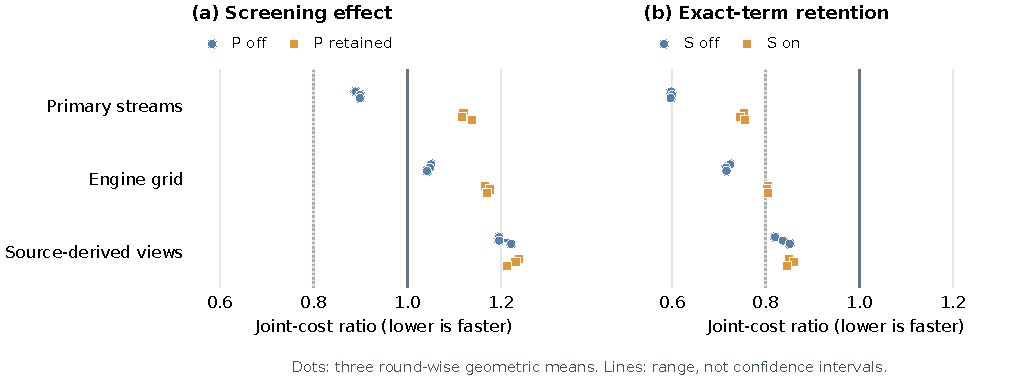
\includegraphics[width=\textwidth]{figures/checking_schedule_v4.pdf}
\caption{Isolating checking costs while preserving the same evidence and solver paths. Each dot is one timing round's equal-weight geometric-mean joint-cost ratio over all inputs in that group; the line shows its three-round range. Screening is compared at each fixed exact-term retention setting, and retention at each fixed screening setting. The $.8$ reference applies to the two registered primary contrasts only. Values below one indicate less total producer-and-receiver work; no interval is a statistical confidence interval.}
\label{fig:checking-factors}
\end{figure*}
\begin{table*}[t]
\centering\small
\caption{All registered factor and bridge comparisons. Entries are median [minimum, maximum] of the three round-wise geometric-mean joint-cost ratios. Original Prepared is lower-only and cannot prove false; Auto changes the simplex strategy. Their cost ratios are descriptive. Source-derived serving starts from saved views, excluding source ingestion.}
\label{tab:checking-factors}\begin{tabular}{lrrr}
\toprule
Contrast & Primary & Engine & Source-derived \\
\midrule
Screening, $P=0$ & 0.899 [0.889, 0.899] & 1.048 [1.042, 1.051] & 1.196 [1.196, 1.222] \\
Screening, $P=1$ & 1.120 [1.118, 1.138] & 1.170 [1.167, 1.177] & 1.231 [1.213, 1.238] \\
Exact retention, $S=0$ & 0.598 [0.597, 0.600] & 0.717 [0.715, 0.724] & 0.837 [0.820, 0.852] \\
Exact retention, $S=1$ & 0.753 [0.746, 0.756] & 0.804 [0.804, 0.805] & 0.849 [0.845, 0.862] \\
Both / original Prepared & 1.449 [1.449, 1.455] & 0.909 [0.899, 0.912] & 1.198 [1.184, 1.199] \\
Both / Auto bridge & 0.996 [0.959, 0.997] & 0.995 [0.994, 0.997] & 0.992 [0.990, 0.997] \\
\bottomrule
\end{tabular}

\end{table*}


All 1,134 plan-streams and 162,000 responses complete, with independent numerical replay and complete source bindings. The four core plans return identical evidence, decisions, routes and native-solver paths. Figure~\ref{fig:checking-factors} therefore isolates checking work rather than a change in which queries get answered. On the primary streams, screening with retained terms has round-wise ratios $1.120$, $1.118$, $1.138$; retaining exact terms with screening has ratios $0.753$, $0.746$, $0.756$. The joint requirement that both factors meet the registered primary engineering target is not supported. Table~\ref{tab:checking-factors} retains all six contrasts and both broader groups. The artifact includes every per-input ratio, prefix, factor interaction and decision comparison, including slow inputs and bridge losses. These are fixed-workload timing observations, not a significance or deployment-generalization claim.

\textbf{Caching changes whether screening pays.} Without retained exact terms, screening has primary ratios $0.889$--$0.899$; after retention, the same screening loses (Fig.~\ref{fig:checking-factors}). Retention without screening gives ratios $0.597$--$0.600$. Across the three primary inputs in each round, screening reduces exact dual checks from 6000 to 3003. With retained terms it saves 11.04--11.41\,s of producer verification, but screening itself costs 17.93--18.35\,s. These component timers explain the observed tradeoff; they are not added again to joint cost. A filter that avoids checks can therefore become uneconomic after those checks have been made cheaper. The broader groups also lose from screening under both retention settings; the evidence does not support screening every workload by default.

The bridge comparisons change answer capabilities as well as execution. On the engine grid, Both gains 15 decided answers and loses three relative to Auto; the primary and source-derived groups have no differences. Relative to lower-only Original Prepared, Both gains 2,438 of 5,400 engine-grid answers and 354 of 600 source-derived answers, with no losses; all 3,000 primary answers already agree. Complete true/false/unknown counts remain in the artifact. Neither bridge isolates a factorial effect.

\begin{table}[t]
\centering\small
\caption{Absolute checking costs on the three primary streams. In each round, joint time and uncompressed response bytes are divided by 3,000 requests; receiver share is receiver time divided by joint time. Entries are medians of three rounds. Joint cost includes the persistent receiver; 1 KiB is 1,024 bytes.}
\label{tab:absolute-checking}
\begin{tabular}{lrrr}
\toprule
Plan & Joint ms/request & Receiver & KiB/request \\
\midrule
$S_0P_0$ & 30.45 & 27.5\% & 30.39 \\
$S_0P_1$ & 18.26 & 45.9\% & 30.39 \\
$S_1P_0$ & 27.36 & 30.9\% & 30.39 \\
$S_1P_1$ & 20.41 & 40.9\% & 30.39 \\
\bottomrule
\end{tabular}
\end{table}



\subsection{History and materialization boundaries}
Earlier matched comparisons give Prepared joint ratios $.738$--$.765$ against Threshold Hot and $.746$--$.806$ against Auto, missing the registered $.8$ target once. Every plan solves once and reuses one dual 999 times. The controls also retain exact terms but check the box first; this comparison cannot isolate preparation.

In the broader 6,000-query threshold grid, Both Histories has joint ratios $.996$--$1.001$ against Threshold Hot and $.993$--$1.000$ against Auto; the target fails. Answers comprise 2,957 true, 2,794 false and 249 unknown. Earlier history serves only 41 queries, all primal points, 38 in one 64-cell region. It gains/loses 2/0 decided answers against Hot and 16/2 against Auto. The losses involve native proposals outside exact feasibility by $2^{-53}$--$2^{-55}$. Verification and receiving cost 87.9\% of joint time; native solving costs 0.173\%. Mean responses contain 51,493 bytes.

At $Q=100$ in the seven-plan grid, Prepared is no slower than Hot in 9/18 cells; its worst median producer ratio is 10.704. With five million source events, rebuilding costs 5.56--6.12\,s, Hot $.140$--$.150$\,s and Prepared $.284$--$.289$\,s. Prepared/Hot joint ratios are 1.580 and 1.619: materialization helps, but additional prepared reuse loses. All raw responses, prefixes and adverse cells remain available.

\subsection{What stronger source information changes}\label{sec:historical}
A retrospective diagnostic retains all 400 historical count/policy pairs at $\Lambda=2$, $\rho=0$, $\alpha=.05$, $\delta=.001$, with full-budget standalone sources. Consistency information~\eqref{eq:consistency} lets OBS certify 99/100 external $2\times2$ queries: group fusion adds none and projected fusion adds one. For learned $2\times2$ queries, OBS/group fusion/projected fusion certify 5/51/66. For external $8\times8$ queries, both fusions certify 100 and standalone sources none; all methods fail on learned $8\times8$ queries. Neither R standalone certifies. A stronger OBS comparator therefore removes one apparent fusion advantage.

These inspected stress tests have generating radii 1.2892 and 1.3248. The $8\times8$ KuaiRec-derived surface~\cite{gao2022kuairec} imposes exposures and query-directed randomized means, so it cannot establish typical gains. A separate census finds no true-radius fusion-only case in 35 generating settings. Complete budgets, assumptions and comparison rows remain available. The fresh-world study avoids query-directed source construction.

\subsection{What limits information from fusion}\label{sec:information-results}
\begin{table}[t]
\centering
\caption{Conservative, lower-budget diagnosis; 240 queries per policy. Finite: the finite optimum fails but the population optimum passes. Pop.: the true effect exceeds $\delta$ but both optima fail. No query is missed solely by numerical optimization.}
\label{tab:fresh}\begin{tabular}{lrrrr}
\toprule
Policy & Cert. & Finite & Pop. & True $\le\delta$\\
\midrule
Metadata & 12 & 33 & 195 & 0\\
R heuristic & 4 & 43 & 190 & 3\\
Robust design & 2 & 0 & 0 & 238\\
\bottomrule
\end{tabular}

\end{table}

All 60 worlds and 1,200 inference configurations complete. Primary fusion certifies 12/240 versus six for the standalone union (OBS six, R zero): six additions, no losses, and world-average gain $0.025$. The registered Hoeffding lower endpoint is $-0.3283$, failing the five-percentage-point target. With 48 worlds its penalty is 35.33 points, requiring over 40.33 points of observed gain; it has little power for modest benefits. The descriptive stratified $t$ interval is $[-0.0249,0.0749]$, standard error $0.0186$. The criterion remains unchanged; nonconfirmation does not prove no benefit.

At the larger randomized budget, projected fusion certifies 15 metadata queries, 16 heuristic queries, and two robust-design selections. Increased randomized traffic does not remove uncertainty about source transfer or the sensitivity radius. Both budgets and all policy families remain in the artifact.


\begin{figure*}[t]
\centering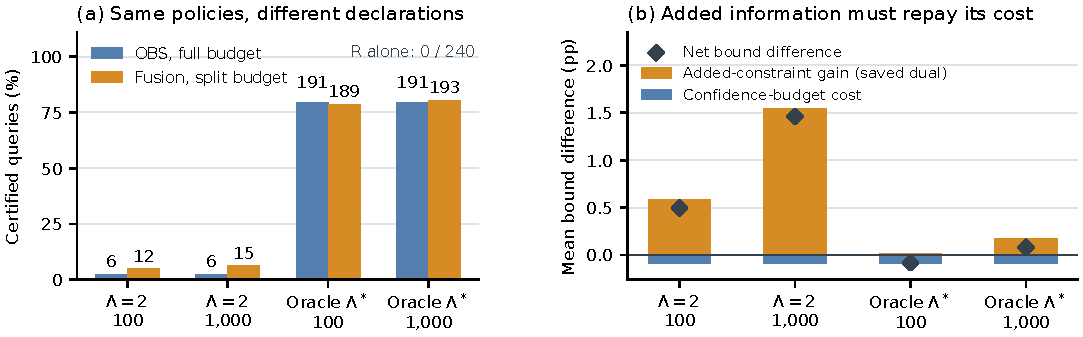
\includegraphics[width=\textwidth]{figures/repaired_information_v4.pdf}
\caption{The same metadata policies under four radius and event-budget settings. (a) Certification rates, with raw counts annotated out of 240 queries from 48 worlds with five count samples each. R denotes the projected-group standalone and certifies none. (b) The saved-dual gain from adding group constraints, minus the observational confidence-budget cost, gives the net bound difference. Values are success-probability percentage points, not policy effects. $n_R/d$ is a nominal event budget; the two budgets are separate sampled streams. The oracle radius uses generating truth.}
\label{fig:sensitivity}
\end{figure*}
% Generated only after independent repaired-program result audit.
\textbf{Finite width or population ambiguity?}
Exact primal--dual certificates give finite and population optima for all three methods on all 2,880 query records. All 960 finite fusion views strictly contain their population counterparts. The latter replace sampling intervals by exact source quantities under the same declared relaxation; they do not assume full-cell transport or latent-model sharpness. Table~\ref{tab:fresh} partitions the conservative, lower-budget results. No finite optimum passes when the returned fusion answer fails. All 240 primary true effects exceed $\delta$: 195 remain blocked by population ambiguity and 33 by the current finite intervals. These categories do not estimate required sample sizes.

Of the 6 additional finite certifications across 2 worlds, 4 queries have a sufficient population standalone source and 2 pass only with population fusion. The latter regime spans 7 worlds (35 repeated queries). The robust design rule retains the reference in 238/240 lower-budget cases. These are diagnoses of the saved worlds, not general frequencies of source complementarity.

\textbf{A tighter declaration can make fusion unnecessary.}
The oracle radii range from 1.0318 to 1.3881. With the same metadata policies and count samples, the low-budget oracle setting certifies 191/240 from OBS and 189/240 from fusion, compared with 6 and 12 at $\Lambda=2$ (Fig.~\ref{fig:sensitivity}). The four settings add/lose 6/0, 9/0, 0/2 and 3/1 certifications relative to the standalone union. Truth supplies the oracle radius; the plot does not learn a defensible declaration from observed data.

\textbf{Why the budget split can lose a certification.}
Replacing $V_F$ by the saved exact dual $D_F$ in~\eqref{eq:gain-cost} gives the achieved-gain decomposition in Fig.~\ref{fig:sensitivity}b; $D_F$ need not be optimal. At the lower budget and oracle radius, mean achieved gain is 0.0114~pp and budget cost 0.0913~pp, leaving -0.0799~pp. These are bound differences, not policy effects. Proposition~\ref{prop:box-face} proves zero optimal gain for 193/240 oracle metadata queries versus 24/240 at $\Lambda=2$; at the larger budget the counts are 36 and 8. The two low-budget certification losses have zero optimal gain: the half-budget box minimizer already satisfies every group constraint. The third loss, at the larger budget, has positive optimal gain smaller than its budget cost. Exact optima rule out missed optimization in all three.

Across all policies and settings, 1309 of 2,880 queries have zero optimal constraint gain, including 674 trivial zero objectives; the nonzero subset has 635/2206 such cases. The randomized budgets are separate count streams. The robust policy changes in 278 of 480 radius-paired records, so its comparison cannot isolate radius alone. Complete strata and all policy families remain in the artifact.


\begin{table}[t]
\centering
\caption{Fresh-study diagnostics. A query violation is a bound above truth. Denominators count views or queries; reused records are dependent.}
\label{tab:coverage}\begin{tabular}{lrrr}
\toprule
Construction & Set misses & Query violations & Refusals\\
\midrule
OBS & 2/1200 & 0/3600 & 0/1200\\
R projected & 0/1200 & 0/3600 & 0/1200\\
Fused projected & 2/1200 & 0/3600 & 0/1200\\
R group score & 4/1200 & 0/3600 & 0/1200\\
Fused group score & 6/1200 & 0/3600 & 0/1200\\
\bottomrule
\end{tabular}

\end{table}

Table~\ref{tab:coverage} separates set coverage from individual answers. The 6,000 synthetic inference views have 14 set misses; no returned bound exceeds its true contrast, no query falsely certifies and no view is refused. All 18,900 repaired proofs (18,000 synthetic, 900 thinned Coat) were independently checked. Seven group-score fusion answers change from certified to unresolved; all projected-method statuses are unchanged. The original 600 design views remain separate, with one set miss and no refusal. These observations do not prove uniform coverage or validate the scientific premises; Theorem~\ref{thm:simultaneous} remains conditional on them.

% Revision-5 comparison; previous frozen table preserved separately.
% Evidence: runs/icde2027/literature/capability_comparison_v3.{md,json}.
% Five data rows, four columns. Uses existing booktabs/array packages and BibTeX keys.
\begin{table*}[t]
\centering
\caption{Documented task scopes and reuse layers; entries are not impossibility claims. O/R denotes observational/randomized data.}
\label{tab:capability-comparison}
\footnotesize
\setlength{\tabcolsep}{3pt}
\renewcommand{\arraystretch}{1.12}
\begin{tabular}{@{}>{\raggedright\arraybackslash}p{.15\textwidth}>{\raggedright\arraybackslash}p{.27\textwidth}>{\raggedright\arraybackslash}p{.28\textwidth}>{\raggedright\arraybackslash}p{.26\textwidth}@{}}
\toprule
Work & Input / assumptions & Task / reuse layer & Guarantee / checked object \\
\midrule
Du et al.~\cite{du2026feasible} & O/R; recoverable non-overlap; known randomization and moment feasibility & Response estimation; joint representation fitting & Experimental moments; observational excess-risk bound \\
Lanners et al.~\cite{lanners2025fusion} & O/R; positivity; confounding and study sensitivity & Sensitivity frontiers; reused nuisance fits & (C)ATE bounds; asymptotic inference \\
Deza et al.~\cite{Deza2026MIPSensitivity} & LP/MILP with finite variable bounds & Changed objective, RHS, matrix; cached duals/tree & Valid lower bounds; conditional gap bound \\
SemViews~\cite{Hassanzadeh2026SemanticViews} & Relation, oracle labels, catalog & New predicates; historical features, fresh certification draws & Per-query precision/recall probability \\
VIPR~\cite{Cheung2017VIPR} & Rational MILP and derivation log & Independent replay of instance-specific derivations & Exact bounds/infeasibility verification \\
Q-BRIDGE & Binary O/R aggregates or iid user blocks; declared sensitivity and group transport & One confidence view; changing policies and margins; checked evidence reuse & Simultaneous coverage of means; exact lower and feasible-upper proofs for the stored LP \\
\bottomrule
\end{tabular}
\end{table*}


\subsection{Real data: inference over user blocks}\label{sec:coat}
Coat contains 290 users, each with 24 self-selected and 16 uniformly randomized ratings from 300 items~\cite{schnabel2016coat}. Success is a rating of at least four; zero means unobserved. Inference concerns the study-user generating distribution under iid users, not 11,600 independent ratings. Each source has a static potential-rating vector, $Y^O_u(a)$ or $Y^R_u(a)$, unaffected by within-source order or panel composition. These vectors need not agree across sources; full-cell transport is additional.

We retain all items and 31 uniform groups defined by gender, jacket type and color. Fifteen fixed queries tilt five metadata features by $0.5$, $1.5$, or $2$ against a uniform reference. Three front-page queries lie outside the moment row space. The primary query doubles the weights of items carrying the \emph{front-page} metadata flag, renormalizes across all 300 items, and compares with the uniform reference. The other twelve cannot demonstrate added population identification from fusion. All twelve $(\Lambda,\rho)$ declarations and five constructions are retained.

\textbf{Original event interface.} Independent auxiliary substreams uniformly select one observed item per source and user, without consulting its rating; $q_a=(16/300)(1/16)=1/300$. The 580 selected events leave 116 empty O cells and 124 empty R cells. All 900 rematerialized query proofs and the 15 separately retained full-cell controls are unresolved; no view is refused.

\textbf{Using every rating.} A separately registered retrospective diagnostic retains O24/R16 panels with the same queries, budgets and declarations. It assumes simple random R16 subsets without replacement, independently of potential ratings and across users. The release describes random/uniform selection; its collection implementation is unavailable to establish these conditions.

O conditional CP uses included users for each item; joint success/failure CP uses $N=290$. Uniform thinning of 24 selected items divides marginal and latent inclusion propensities by 24, preserving their ratio and conditional rating distribution. Thus $\Lambda$ retains its meaning, while full inclusion supplies stronger consistency information. Changes from thinning are not solely sampling-variance effects.

For R group $G_j$, let $M_{uj}=|R_u\cap G_j|$. An active user contributes its mean binary rating over these sampled items. Conditional on $M_{uj}>0$, its expectation is the user's uniform group mean; activity is independent of potential ratings. Conditional on the active count, scores are iid in $[0,1]$. All groups contain multiple items, so~\eqref{eq:eb} uses 72--290 active users and variance denominator $n_j-1$. Item histograms cannot recover this variance. The projected alternative uses per-item CP over included users. Each retains its fixed budget and union-bound coverage.

The matrix is unchanged. Exact user-score moments and interval propagation feed the normalized-row mapping in~\eqref{eq:represented}. The final full-panel construction uses the same user blocks, groups, queries and source declarations; changing the numerical representation supplies no new observations or evidence for transport.

\begin{table}[t]
\centering
\caption{Coat primary-query lower bounds in success-probability units at $\Lambda=2$, $\rho=0$, $\alpha=.05$. Both protocols use 290 users. Full panels change the statistics and inclusion-consistency information. R full-cell control additionally assumes full-cell transport.}
\label{tab:coat-blocks}\begin{tabular}{lrr}
\toprule
Construction & \shortstack{One item\\per source} & \shortstack{Full user\\blocks}\\
\midrule
OBS & $-0.04784$ & $-0.03729$\\
R group & $-0.01261$ & $-0.01502$\\
R projected & $-0.04787$ & $-0.03402$\\
Fusion group & $-0.01295$ & $-0.01193$\\
Fusion projected & $-0.04782$ & $-0.03132$\\
R full-cell control & $-0.04768$ & $-0.03077$\\
\bottomrule
\end{tabular}

\end{table}

% Generated from independently audited fixed-data V5 repair.
All 915 full-panel lower-bound answers remain unresolved, with no refused view. At the primary declaration, group fusion gives $-0.01193$ versus $-0.01502$ for full-budget R group: a 0.309-percentage-point improvement in the bound, not a measured policy effect. Neither passes $\delta=.001$. Table~\ref{tab:coat-blocks} retains every source construction. The independent audit reconstructs user-level statistics and all 61 views, 915 proofs and 15 direct controls. It does not establish the scientific source assumptions.


% Generated from all 15 independently audited direct controls.
The full-cell premise also permits direct randomized scores, averaged over all 16 ratings within each user, followed by a one-sided Hoeffding bound with $N=290$ for each fixed query. The primary estimate is $0.00371$ and its lower bound $-0.06452$. None of the 15 controls passes its margin. These per-query bounds do not support adaptive selection; failure to certify does not establish zero effect or validate transport.


\subsection{Catalogue policy queries}\label{sec:catalogue-workflow}
% Working methods text for the fixed V5 workflow; no result is asserted here.
\textbf{A catalogue workload with ordinary caching.}
To test what remains after ordinary caching, a retrospective workload combines all ten pairs of the same five attributes: front-page flag, men, fleece, waterproof and black. Item $a$ receives weight $m_1^{h_1(a)}m_2^{h_2(a)}$, normalized over 300 items, for binary attributes $h_1,h_2$ and multipliers $m_1,m_2\in\{.5,1,2\}$. Omitting only $(1,1)$ gives 80 positions in fixed serpentine order, including duplicates. Repeating them at margins $0$, $.001$ and $.01$ gives 240 requests per view. Metadata alone generates these policies; Eq.~\eqref{eq:policy-rounding} transfers their stored bounds to ideal contrasts.

On each of the five unchanged primary views, three executors share a full-capacity objective cache and the same persistent receiver. A cache hit rebinds evidence to the current margin; if still undecided, execution resumes and valid stronger evidence is merged. We compare current prepared execution with screening off, an optimized exact reference with the same candidate schedule, and full native hot-start LP with the optimized checker. The exact reference uses direct box arithmetic, skips zero-multiplier rows and uses sparse residual corrections when its fixed operation-count rule favors them. Native hot-start retains its basis but no cross-objective proof candidates. It reoptimizes every request that the common cache cannot decide, using the initial witness as an upper-bound fallback. These are implementation controls, not new inference rules.

All $3\times5\times240$ responses undergo quality verification before three fixed timing rounds. Each stream starts fresh; method order rotates. Joint cost follows Section~\ref{sec:design}, also charging ideal-policy transfer. Cold verification, prefixes, first occurrences, duplicates, bytes and retained state are recorded separately.

Information comparisons pool checked bounds from all executors and repeated positions for each distinct objective--margin pair, uniformly across views. Fusion-only certification requires an ideal lower bound above the margin and neither corresponding standalone view to certify; unavailable references are separate. Execution comparisons retain each method's own answers. The engineering target requires no lost decided answer and a five-view geometric-mean optimized/current joint-cost ratio at most $.9$ in every round. Repeats and overlapping views are not independent populations.

% Generated from both complete independently audited workflow stages.

\begin{table}[tb]
\centering\small
\caption{Catalogue decisions and costs. C/O/H denote current prepared, optimized exact and native hot execution. Decided counts are out of 240 quality requests; no answer is true. Each time is joint cost divided by 240, then median over three rounds, in ms/request. Native hot has different answer quality. Complete round-wise costs and ratios remain in the artifact.}
\label{tab:catalogue-workflow}
\begin{tabular}{lrrrr}
\toprule
View & Decided C/O/H & C & O & H \\
\midrule
OBS & 240/240/240 & 8.20 & 7.94 & 8.07 \\
R group & 197/197/174 & 13.68 & 12.57 & 14.96 \\
R projected & 163/163/163 & 16.83 & 15.60 & 15.33 \\
Fusion group & 219/219/185 & 12.33 & 11.82 & 15.07 \\
Fusion projected & 208/208/171 & 12.91 & 12.41 & 14.69 \\
\bottomrule
\end{tabular}
\end{table}


The sequence contains 50 distinct objectives and 150 objective--margin pairs per view. Its ideal objective rank is 14 and its represented rank 15; 12 distinct objectives lie in the moment row space under either encoding. The error transfer changes no answer. No view certifies a positive policy effect, so neither fusion-only information target is supported.

Table~\ref{tab:catalogue-workflow} reports all five views. Current and optimized execution agree on all 1,200 quality requests. Their three round-wise geometric-mean joint ratios are $0.960$, $0.941$, $0.953$; the registered ten-percent engineering target is not supported. Native hot loses 98 decided answers and gains 4 relative to current execution; its cost is therefore not an equal-service comparison. False answers identify feasible counterexamples to a robust guarantee, not negative measured policy effects. Complete three-round outcomes, prefixes, first occurrences and duplicates remain in the artifact.

Optimized execution is slower than current in 3/15 view--rounds and retains more exact-state payload in every view. These are recorded Python payload estimates, not isolated RSS measurements. Native hot is faster than optimized in all three R projected rounds, with the same decisions there.


\section{Related Work and Scope}\label{sec:related}
Table~\ref{tab:capability-comparison} distinguishes statistical objects, reuse mechanisms and numerical certificates. Binary density-ratio and conditional-moment bounds supply our statistical building blocks~\cite{dorn2025dvds,ishikawa2026convex}; source integration can also exploit differences in overlap~\cite{jiang2024overlap}. Our finite-table interface does not establish latent-model sharpness.

\textbf{Causal and uncertain database queries.} HypDB adjusts biased aggregates~\cite{salimi2018hypdb}; ZaliQL implements matching~\cite{salimi2017zaliql}; CaRL defines relational causal units~\cite{salimi2020carl}; CauSumX explains views with causal patterns~\cite{youngmann2024causumx}. Uncertainty-annotated databases propagate conservative relational information~\cite{Feng2019UADB}. Our object instead stores correlated mean constraints. Unlike SemViews' fresh predicate-certification draws~\cite{Hassanzadeh2026SemanticViews}, all objectives here concern one covered target vector. We operate over encoded columns, without general SQL or automatic causal discovery.

\textbf{Proofs and trust.} Safe approximate-dual bounds~\cite{Neumaier2004SafeBounds} and dual-based warm starts~\cite{Marcucci2021WarmStart} complement the numerical precedents in Table~\ref{tab:capability-comparison}. IntegriDB addresses a stronger cryptographic database authentication setting~\cite{Zhang2015IntegriDB}; our hash binds a proof to a caller-trusted view without authenticating the source table or its freshness.

\textbf{Limits.} The implementation assumes binary outcomes and known standardized target weights; continuous covariates, estimated weights and dependent interactions need additional methods. Scientific assumptions and statistical quantile routines remain trusted. Fine partitions can leave intervals uninformative, and prepared reuse may cost more than reoptimization for distant objectives. Exact proofs certify the represented optimization problem, not those scientific premises.

\textbf{Data ethics.} This study only performs secondary analysis of publicly released benchmarks under their release terms, without recruiting or interacting with participants. On this basis, no institutional ethics review or additional participant consent was obtained for this work. We do not claim a formal institutional exemption or verification of the original collection's approval and consent procedures.

The local artifact includes source snapshots, protocols, complete results, input provenance and a standard-library proof checker. No public artifact URL is currently available.

\section{Conclusion}
Q-BRIDGE connects a two-source confidence view to independently checkable policy queries. Holding answers and solver paths fixed separates the benefit of retaining exact terms from the cost of screening candidates; on the primary streams, retention helps, and screening changes from a saving to a loss once those terms are retained. Earlier history contributes little across the broader grid. Information diagnostics separate constraint gain, confidence-budget cost and population ambiguity. A feasible point on the box's minimizing face certifies zero optimal gain from additional constraints. These results delimit when computation can be reused and when a policy decision instead needs stronger information.

\section*{Acknowledgments and AI Usage Declaration}
OpenAI Codex assisted with drafting and mathematical exposition in Sections I--VIII, code and experiment development for Sections III--VI, and generation of the figures. It also assisted with source retrieval and editing throughout the article. Computational claims were checked against saved artifacts and citations against primary sources. The authors are responsible for correctness, originality and the final submission.

\bibliographystyle{IEEEtran}
\bibliography{revision2_references}
\end{document}
